\documentclass[12pt]{article}

\usepackage[a4paper, total={170mm,257mm}, left=20mm, top=20mm]{geometry}
\usepackage{mathtools}
\usepackage{amsfonts}
\usepackage{graphicx}

\title{Solving Differential Equation Using Finite Element Method}
\author{Piotr Magiera}
\date{February 2022}

\begin{document}

\maketitle

\section{Introduction}

The aim of this paper is to use Finite Element Method to solve the equation
\[\frac{d^2 u}{dx^2}=4\pi G\rho (x)\]
with following assumptions:
\[u(0)=5,\]
\[u(3)=4,\]
\[\rho(x)=\begin{cases} 
      0 & x \in \langle0, 1 \rangle\\
      1 & x \in (1, 2 \rangle\\
      0 & x \in (2, 3 \rangle\\
   \end{cases},\]
\[u: \langle 0, 3 \rangle \to \mathbb{R},\]
\[G = 6.67 * 10^{-11}.\]


\section{Weak form of the equation}


Let $U=\{f\in H^1(0, 3): f(0)=f(3)=0\}$. Function $u$ satisfies the equation if and only if for any $v \in U$
\[\int_0^3 u'' v dx=\int_0^3 4 \pi G \rho v dx.\]
Using integration by parts we obtain
\[u'v\Big|_0^3 - \int_{0}^3 u' v' dx =4 \pi G \int_0^3 \rho v dx.\]
Since $v \in U$, $u'v\Big|_0^3=0$. Moreover, $\rho(x) \neq 0 \iff x \in \langle 1, 2 \rangle$ 
and  $\rho(x) = 1$ for $x \in \langle 1, 2 \rangle$, hence
\begin{equation}- \int_0^3 u' v' dx = 4 \pi G \int_1^2 v dx.\end{equation}


\indent
Let us define functions $\bar u$ and $w$ such that 
\begin{equation} u = \bar u + w \end{equation} 
and $w \in U$. Therefore $w(0)=w(3)=0$, which implies 
$\bar u(0) = u(0) = 5$ and $\bar u(3) = u(3) = 4$. According to the above remark, we define
\begin{equation} \bar u(x) = 5 - \frac{x}{3}.\end{equation}

\pagebreak[4]

\noindent
Applying (2) and (3) we can rewrite (1) as
\[\int_0^3 (\frac{1}{3} - w') v' dx = 4 \pi G \int_1^2 v dx\]
which is equivalent to weak form of the main equation
\begin{equation} - \int_0^3 w' v' dx = 4 \pi G \int_1^2 v dx -  \frac{1}{3} \int_0^3 v' dx.\end{equation}


\section{Discretization}


We will denote by n the number of subdomains the $\langle0, 3 \rangle$ set will be divided in and by $h = \frac{3}{n}$ the length of each subdomain. Furthermore, let: 

\[\forall i \in \{0, ..., n\}: x_i = h*i,\] 

\[\forall i \in \{1, ..., n-1\}:
  e_i (x)=\begin{cases} 
      \frac{x - x_{i-1}}{x_i - x_{i-1}} & \text{for } x \in (x_{i-1}, x_i\rangle\\
      \frac{x_{i+1} - x}{x_{i+1} - x_i} & \text{for } x \in  (x_i, x_{i+1})\\
      0 & \text{otherwise}
   \end{cases}.\]

% cheating block comment
\iffalse
\[e_0 (x)=\begin{cases} 
      \frac{x_{1} - x}{x_{1} - x_0} & \text{for } x \in  \langle x_0, x_1)\\
      0 & \text{otherwise}
   \end{cases},\]

\[e_n (x)=\begin{cases} 
      \frac{x - x_{n-1}}{x_n - x_{n-1}} & \text{for } x \in (x_{n-1}, x_n\rangle\\
      0 & \text{otherwise}
   \end{cases}.\]
\fi
%

\indent
The idea behind discretization is to approximate infinite-dimensional linear space $U$ with finite-dimensional space $V \subset U$.
Since we have Dirichlet boundary conditions on both sides of the domain, let $V=Lin\{e_1, ..., e_{n-1}\}$. Now we have replaced the equation (4) with its finite-dimensional version where $w, v \in V$.


\section{Matrix form of the problem}


The fact that $w \in V$ implies that $w = \sum_{i=1}^{n-1} \alpha_i e_i$. With the notation $B(w, v) = - \int_0^3 w' v' dx$,
$\bar L(v)=4 \pi G \int_1^2 v dx -  \frac{1}{3} \int_0^3 v' dx$, we can write (4), taking $v=e_j$ for $j \in \{1, ..., n-1\}$, in the form

\[\forall j \in \{1, ..., n-1\}: B(\sum_{i=1}^{n-1} \alpha_i e_i, e_j) = \bar L(e_j),\]
which is equivalent to

\begin{equation} \forall j \in \{1, ..., n-1\}: \sum_{i=1}^{n-1} \alpha_i B(e_i, e_j) = \bar L(e_j). \end{equation}
The set of equations (5) can be represented in matrix form as
\begin{equation}
  \begin{bmatrix}
	B(e_1, e_1) & B(e_2, e_1) & \cdots & B(e_{n-1}, e_1) \\
	B(e_1, e_2) &  B(e_2, e_2) & \cdots & B(e_{n-1}, e_2) \\
	\vdots  & \vdots  & \ddots & \vdots  \\
	B(e_1, e_{n-1}) &  B(e_2, e_{n-1}) & \cdots &  B(e_{n-1}, e_{n-1})
  \end{bmatrix}  
 \*
  \begin{bmatrix}
	\alpha_1 \\
	\alpha_2 \\
	\vdots \\
	\alpha_{n-1} \\
  \end{bmatrix}
=
  \begin{bmatrix}
	\bar L(e_1) \\
	\bar L(e_2) \\
	\vdots \\
	\bar L(e_{n-1}) \\
  \end{bmatrix}.
\end{equation}

\pagebreak[4]

\section{Simplification of the matrix form}


It is easily seen that $B(e_i, e_j) \neq 0 \iff |i-j| \leq 1$. Since 
\[e_i'(x) = 
  \begin{cases}
	\frac{1}{h} & x \in (x_{i-1}, x_i) \\
	- \frac{1}{h} & x \in (x_i, x_{i+1}) \\
	0 & x \in (-\infty, x_{i-1}) \cup (x_{i+1}, +\infty)
  \end{cases},\] 
we get constant values:
\[a = B(e_i, e_i) = - \int_{x_{i-1}}^{x_{i+1}} \frac{1}{h^2}dx,\]
\[b = B(e_i, e_j) = \int_{x_i}^{x_{i+1}} \frac{1}{h^2}dx \text{ for } |i-j| = 1.\]
Obviously
\[\forall i \in \{1, ..., n-1\}: \int_0^3 e_i'dx = 0 \implies \bar L(e_i) = 4 \pi G \int_1^2 v dx.\]


We can now rewrite (6) as
\begin{equation}
  \begin{bmatrix}
	a & b & 0 & 0 & \cdots & \cdots & \cdots &\cdots & \cdots \\
	b & a & b & 0 & \ddots & \ddots & \ddots & \ddots & \vdots \\
	0 & b & a & b & \ddots & \ddots &  \ddots & \ddots & \vdots \\
	\vdots & \ddots & \ddots & \ddots & \ddots & \ddots & \ddots & \ddots & \vdots \\
	\vdots & \ddots & \ddots & \ddots & \ddots & b & a & b & 0 \\
	\vdots & \ddots & \ddots & \ddots & \ddots & 0 & b & a & b \\
	0 & \cdots & \cdots & \cdots & \cdots & 0 & 0 & b & a
  \end{bmatrix}  
 \*
  \begin{bmatrix}
	\alpha_1 \\
	\alpha_2 \\
	\vdots \\
	\alpha_{n-1} \\
  \end{bmatrix}
=
  \begin{bmatrix}
	\bar L(e_1) \\
	\bar L(e_2) \\
	\vdots \\
	\bar L(e_{n-1}) \\
  \end{bmatrix}.
\end{equation}
 

\section{Plot of the solution}

In the figure 1 we can see plot of the solution obtained using Python script.

\begin{figure}[h]
    \centering
    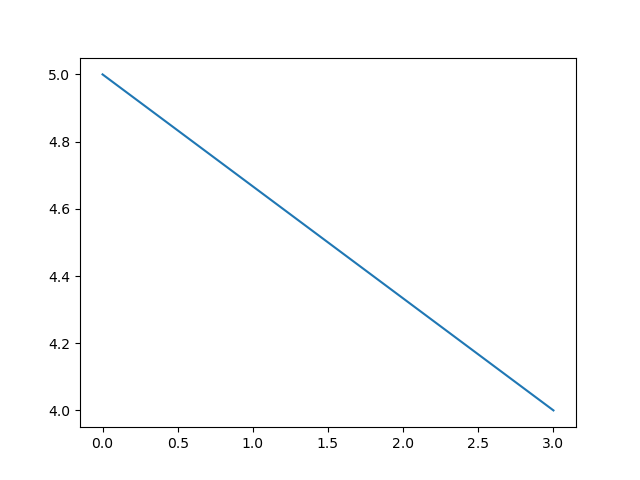
\includegraphics[width=0.5\textwidth]{plot}
    \caption{Plot of $y=u(x)$}
\end{figure}


\end{document}
